\documentclass[
  bibliography=totoc,     % Literatur im Inhaltsverzeichnis
  captions=tableheading,  % Tabellenüberschriften
  titlepage=firstiscover, % Titelseite ist Deckblatt
]{scrartcl}

% Paket float verbessern
\usepackage{scrhack}

% Warnung, falls nochmal kompiliert werden muss
\usepackage[aux]{rerunfilecheck}

% unverzichtbare Mathe-Befehle
\usepackage{amsmath}
% viele Mathe-Symbole
\usepackage{amssymb}
% Erweiterungen für amsmath
\usepackage{mathtools}

% Fonteinstellungen
\usepackage{fontspec}
% Latin Modern Fonts werden automatisch geladen
% Alternativ zum Beispiel:
%\setromanfont{Libertinus Serif}
%\setsansfont{Libertinus Sans}
%\setmonofont{Libertinus Mono}

% Wenn man andere Schriftarten gesetzt hat,
% sollte man das Seiten-Layout neu berechnen lassen
\recalctypearea{}

% deutsche Spracheinstellungen
\usepackage{polyglossia}
\setmainlanguage{german}


\usepackage[
  math-style=ISO,    % ┐
  bold-style=ISO,    % │
  sans-style=italic, % │ ISO-Standard folgen
  nabla=upright,     % │
  partial=upright,   % ┘
  warnings-off={           % ┐
    mathtools-colon,       % │ unnötige Warnungen ausschalten
    mathtools-overbracket, % │
  },                       % ┘
]{unicode-math}

% traditionelle Fonts für Mathematik
\setmathfont{Latin Modern Math}
% Alternativ zum Beispiel:
%\setmathfont{Libertinus Math}

\setmathfont{XITS Math}[range={scr, bfscr}]
\setmathfont{XITS Math}[range={cal, bfcal}, StylisticSet=1]

% Zahlen und Einheiten
\usepackage[
  locale=DE,                   % deutsche Einstellungen
  separate-uncertainty=true,   % immer Fehler mit \pm
  per-mode=symbol-or-fraction, % / in inline math, fraction in display math
]{siunitx}

% chemische Formeln
\usepackage[
  version=4,
  math-greek=default, % ┐ mit unicode-math zusammenarbeiten
  text-greek=default, % ┘
]{mhchem}

% richtige Anführungszeichen
\usepackage[autostyle]{csquotes}

% schöne Brüche im Text
\usepackage{xfrac}

% Standardplatzierung für Floats einstellen
\usepackage{float}
\floatplacement{figure}{htbp}
\floatplacement{table}{htbp}

% Floats innerhalb einer Section halten
\usepackage[
  section, % Floats innerhalb der Section halten
  below,   % unterhalb der Section aber auf der selben Seite ist ok
]{placeins}

% Seite drehen für breite Tabellen: landscape Umgebung
\usepackage{pdflscape}

% Captions schöner machen.
\usepackage[
  labelfont=bf,        % Tabelle x: Abbildung y: ist jetzt fett
  font=small,          % Schrift etwas kleiner als Dokument
  width=0.9\textwidth, % maximale Breite einer Caption schmaler
]{caption}
% subfigure, subtable, subref
\usepackage{subcaption}

% Grafiken können eingebunden werden
\usepackage{graphicx}
% größere Variation von Dateinamen möglich
\usepackage{grffile}

% schöne Tabellen
\usepackage{booktabs}

% Verbesserungen am Schriftbild
\usepackage{microtype}

% Literaturverzeichnis
\usepackage[
  backend=biber,
]{biblatex}
% Quellendatenbank
\addbibresource{lit.bib}
\addbibresource{programme.bib}

% Hyperlinks im Dokument
\usepackage[
  unicode,        % Unicode in PDF-Attributen erlauben
  pdfusetitle,    % Titel, Autoren und Datum als PDF-Attribute
  pdfcreator={},  % ┐ PDF-Attribute säubern
  pdfproducer={}, % ┘
]{hyperref}
% erweiterte Bookmarks im PDF
\usepackage{bookmark}

% Trennung von Wörtern mit Strichen
\usepackage[shortcuts]{extdash}

\author{%
  Jan Philipp Jäkel\\%
  \href{mailto:jan.jaekel@tu-dortmund.de}{jan.jaekel@tu-dortmund.de}%
  \texorpdfstring{\and}{,}%
  Piet Hoffmann\\%
  \href{mailto:piet.hoffmann@tu-dortmund.de}{piet.hoffmann@tu-dortmund.de}%
}
\publishers{TU Dortmund – Fakultät Physik}


\subject{V402}
\title{Die Dispersion am Glasprisma}
\date{
  \begin{align}
    \text{Durchführung: } & \text{15.5.2018} & \hspace{3em} & \text{Abgabe: 22.5.2018} \notag
%\\  \text{Korrektur: } & \text{24.4.2018} & \hspace {3em} & \notag
  \end{align}
}
\begin{document}

\maketitle
\thispagestyle{empty}
\tableofcontents
\newpage

\section{Theorie}
\label{sec:Theorie}
Licht kann als elektromagnetisch Welle verstanden werden.
Dringt eine Lichtwelle in durchsichtige Materie ein, so wechsel wirkt diese mit dem E-Feld der Elektronen.
Daraus resultiert eine Geschwindigkeitsänderung.
Die Geschwindigkeit des Lichts ist, aufgrund dieses Vorgangs, im Medium geringer als die Vakuum-Lichtgeschwindigkeit.
Licht, welches schräg von einem Medium ins andere übergeht, erfährt an der Grenzfläche durch den beschriebenen Vorgang eine Richtungsänderung.
Dieses Phänomen wird als Brechung bezeichnet.
Der Brechungsindex $n$ ist als das Verhältniss der beiden Geschwindigkeiten definiert:
\begin{equation}
  n= \frac{c_1}{c_2} .
\end{equation}
Die Lichtgeschwindigkeit im Medium ist auch von der Frequenz abhängig.
Der Brechungsindex ist demnach auch von der Frequenz des Lichts beziehungsweise der Wellenlänge $\lambda$ abhängig.
Diese Abhängigkeit wird Dispersion gennant.
In diesem Experiment ist die Dispersionskurve
\begin{equation}
  n= f(\lambda)
\end{equation}
von Interesse.
\subsection{Erklärung der Brechung nach dem Huygenschen Prinzip}
Licht erfährt bei dem Übergang in ein optisch dichteres oder dünneres Medium eine Richtungsänderung, diese kann durch Winkel ausgedrückt werden.
Trifft ein Lichtstrahl unter dem Winkel $\alpha$ auf eine Grenzfläche erfährt dieser eine Richtungsänderung und breitet sich unter dem Winkel $\beta$ in dem neuen Medium aus.
Nach dem Huygenschen Prinzip kann jeder Punkt einer bestehenden Wellenfläche als Zentrum einer kugelförmigen Elementarwelle verstanden werden.
Aus der Einhüllenden der Elemntarwellen bildet sich dann die neue Wellenfront.
Berücksichtigt man die erwähnten Winkelabhängigkeiten, dann kann der Brechungsindex in der Form
\begin{equation}
  \label{eq:snell}
  n = \frac{\sin(\alpha)}{\sin(\beta)}
\end{equation}
hergeleitet werden.
Die Gleichung \eqref{eq:snell} wird als Snellius-Brechungsgesetz bezeichnet.
\subsection{Ableitung der Disspersionsgleichung}
Nach Maxwells Theorie kann die Feldstärke einer Elektromagnetischen Welle durch
\begin{equation}
  E = E_0 \exp(i\omega t)
\end{equation}
beschrieben werden.
Damit lässt sich folgende Differentialgleichung der Bewegung formulieren:
\begin{equation}
  m_h \frac{d^2 x_h}{dt^2} +f_h \frac{d x_h}{dt} + a_h x_h = q_h E_0 \exp(i\omega t)  .
\end{equation}
Die Differentialgleichung kann umgeschrieben werden indem $x_h$ durch die Polarisation ersetzt wird:
\begin{equation}
  \label{eq:schwing}
  \frac{d^2 P_h}{dt^2} +\frac{f_h}{m_h} \frac{d P_h}{dt} + \frac{a_h}{m_h} P_h = \frac{N_q q_h^2}{m_h} E_0 \exp(i\omega t)  .
\end{equation}
Die Gleichung\eqref{eq:schwing} ist die Differentialgleichung einer erzwungenen Schwingung.
Diese hat die Lösung
\begin{equation}
  P_h =\frac{1}{\omega_h ^2 -\omega ^2 + i\frac{f_h}{m_h}\omega}\frac{N_q q_h^2}{m_h} E_0 \exp(i\omega t) .
\end{equation}
Die Gesamte Polarisation beträgt
\begin{equation}
  \label{eq:pol}
  P=\sum_{h} \frac{1}{\omega_h ^2 -\omega ^2 + i\frac{f_h}{m_h}\omega}\frac{N_q q_h^2}{m_h} E_0 \exp(i\omega t) .
\end{equation}
Die Polarisation ist gleich der dielektrischen Verschiebung in Materie vermindert um die dielektrische Verschiebung im Vakkum.
Damit kann Gleichung\eqref{eq:pol} umgeschrieben werden zu
\begin{equation}
  (\tilde{\varepsilon} -1)\varepsilon_0 = \sum_{h} \frac{1}{\omega_h ^2 -\omega ^2 + i\frac{f_h}{m_h}\omega}\frac{N_q q_h^2}{m_h} .
\end{equation}
Durch die abgeleitete Maxwellsche Relation
\begin{equation}
  \tilde{n}=\varepsilon
\end{equation}
kann der Zusammenhang zwischen Brechungsindex und Lichtfrequenz hergestellt werden.
Es folgt:
\begin{equation}
  \label{eq:n}
  \tilde{n} =  1 + \sum_{h} \frac{1}{\omega_h ^2 -\omega ^2 + i\frac{f_h}{m_h}\omega}\frac{N_q q_h^2}{m_h \varepsilon_0} .
\end{equation}
Dabei ist $\tilde{n}$ eine komplexe Größe der Form
\begin{equation}
  \tilde{n} = n(1 - ik) ,
\end{equation}
wobei $k$ die Absorbationskonstante von Licht in Materie darstellt.
Der Verlauf der Dispersionskurve wird für
\begin{equation}
  n^2 k \approx 0
\end{equation}
betrachtet.
Die Gleichung\eqref{eq:n} geht dann über in
\begin{equation}
  n^2 (\omega) = 1 + \sum_{h} \frac{N_h q_h ^2}{\varepsilon_0 m_h}\frac {1}{\omega ^2 -\omega_h ^2} .
\end{equation}
Aufgrund der Messbarkeit wird $\omega$ durch $\lambda$ ersetzt.
Damit folgt:
\begin{equation}
  n^2 (\lambda) = 1 + \sum_{h} \frac{N_h q_h ^2}{4 \pi^2 c^2 \varepsilon_0 m_h}\frac{\lambda^2\lambda_h ^2}{\lambda^2 - \lambda_h ^2} .
\end{equation}
Wenn die Betrachtete Materie nur die Absorptionsstelle $\lambda_1$ aufweist,

\noindent dann gilt für $\lambda << \lambda_1$
\begin{equation}
  \label{eq:a}
  n(\lambda) = 1 + \frac{N_1 q_1 ^2 \lambda_1 ^2}{4 \pi^2 c^2 \varepsilon_0 m_1}(1 + (\frac{\lambda_1}{\lambda})^2 + (\frac{\lambda_1}{\lambda})^4 + ...)
\end{equation}
und für $\lambda >> \lambda_1$
\begin{equation}
  \label{eq:b}
  n(\lambda) = 1 - \frac{N_1 q_1 ^2 }{4 \pi^2 c^2 \varepsilon_0 m_1}(\lambda^2+ \frac{\lambda^4}{\lambda_1 ^2} + \frac{\lambda^6}{\lambda_1 ^4} + ...)  .
\end{equation}
Damit entstehen die beiden Dispersionskurven in Abbildung \ref{fig:disp}.
\begin{figure}[H]
  \centering
  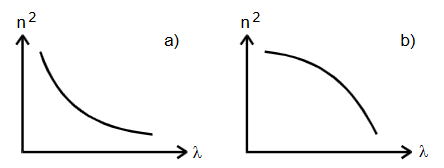
\includegraphics{content/disp.png}
  \caption{Gestalt der Dispersionskurven a) nach Gleichung\eqref{eq:a} und b) nach Gleichung\eqref{eq:b}\cite{v402}.}
  \label{fig:disp}
\end{figure}
\noindent Die dargestellten Kurven beschreiben die normale Dispersion.
Nimmt $n$ mit wachsender Wellenlänge $\lambda$ zu, dann liegt abnormale Dispersion vor.

\section{Durchführung}
\label{sec:Durchführung}
Der Aufbau ist in Abbildung \ref{fig:spek} dargestellt.
\begin{figure}[H]
  \centering
  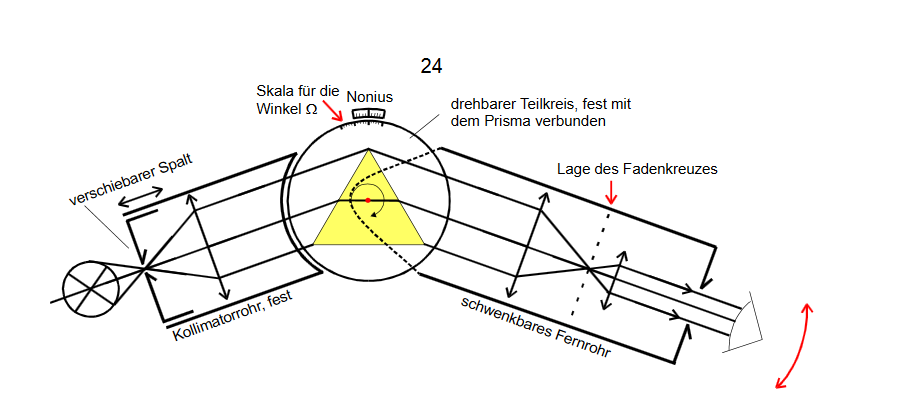
\includegraphics[width=\textwidth]{content/pris_spek.png}
  \caption{Schematische Darstellung eines Prismen-Spektralapparats\cite{v402}.}
  \label{fig:spek}
\end{figure}
\noindent Am Ende des Kollimatorrohrs befindet sich eine HgCd-Spektrallampe.
Das Licht, welches von dieser ausgeht, fällt durch einen Spalt und eine Sammellinse auf ein Glasprisma und wird dort gebrochen.
Das verwendete Prisma ist aus Schwerflint
Nach seiner Brechung gelangt das Licht in ein Fernrohr.
Die Objektivlinse entwirft ein reelles Spaltbild in ihrer Brennebene.
Zur genauen lokalisierung des Spaltbildes ist dort ein Fadenkreuz aufgetragen.
Durch Schwenken um die Goniometerachse kann dann das Fadenkreuz mit dem Spaltbild zur Deckung gebracht werden.
\subsection{Bestimmung der Richtungsänderung des Strahls}
Der $\eta$-Winkel beschreibt die Richtungsänderung des einfallenden Strahls.
Der Strahlengang von dem gebrochenen und dem reflektiertem Strahl sollen parallel verlaufen.
Dies kann realisiert werden, wenn das Prisma gleichschenklig ist und der Strahlengang symmetrisch ist.
Damit ein symmetrischer Strahlengang gefunden werden kann, wird das Prisma so lange um die Goniometerachse geschwenkt bis das reflektierte Spaltbild mit dem gebrochenen übereinstimmt.
Mit dem reflektiertem Spaltbild werden so die Spektrallinien der Lichtquelle abgefahren.
Dabei wird die Winkelstellung des Fernrohrs als auch die Farbe der Spektrallinie notiert.
Danach wird die Messung bei spiegelsymmetrischer Stellung des Prismas wiederholt.
Die erforderliche Prismenstellung ist in Abbildung \ref{fig:eta} schematisch dargestellt.
\begin{figure}[H]
  \centering
  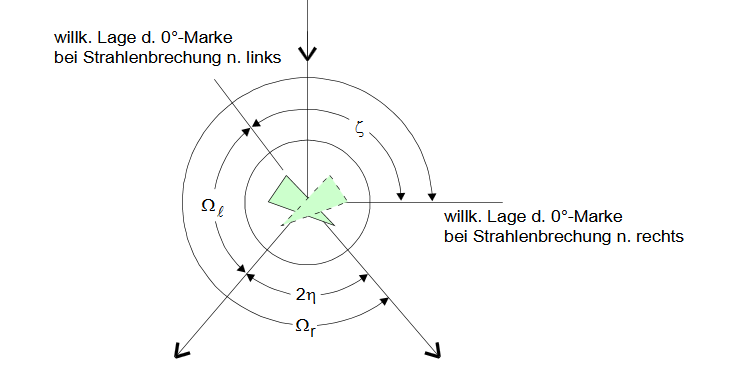
\includegraphics[width=\textwidth]{content/eta.png}
  \caption{Darstellung der Messgrößen $\Omega_l$ und $\Omega_r$ in Abhängigkeit der Prismenstellungen\cite{v402}.}
  \label{fig:eta}
\end{figure}
\noindent Der Winkel $\eta$ kann dann mit
\begin{equation}
  \label{eq:eta}
  \eta = 180 -(\Omega_r - \Omega_l)
\end{equation}
bestimmt werden.
\subsection{Bestimmung des Brechungswinkels}
Das Prisma wird mit seinen brechenden Kanten auf das Kollimatorrohr ausgerichtet.
Das Licht wird an der Prismenoberfläche reflektiert.
Die Reflektionswinkel, dargestellt in Abbildung \ref{fig:phi}, werden mit dem Fernrohr bestimmt.
\begin{figure}[H]
  \centering
  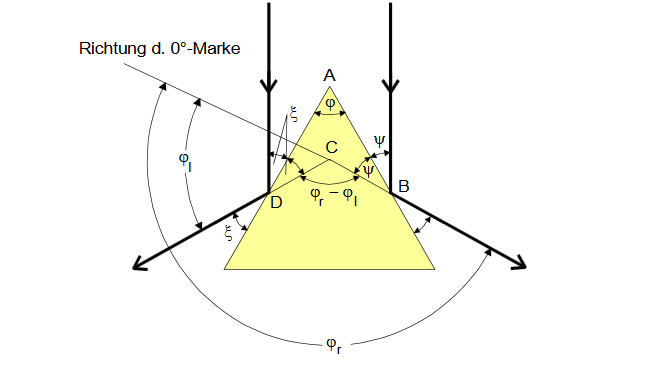
\includegraphics[width=\textwidth]{content/phi.png}
  \caption{Skizze zur Bestimmung des Winkels $\phi$ zwischen den brechenden Oberflächen\cite{v402}.}
  \label{fig:phi}
\end{figure}
\noindent Die Messung wird für sechs verschiedene Prismenstellungen wiederholt.
Der Brechungswinkel $\phi$ kann dann wie folgt berechnet werden:
\begin{equation}
  \label{eq:phi}
  \phi = \frac{1}{2}(\phi_r -\phi_l) .
\end{equation}

\section{Auswertung}
\label{sec:Auswertung}
Die Messwerte für den Winkel $\phi$ des Prismas sind in Tabelle \ref{tab:phimess} aufgetragen.
\begin{table}[H]
    \caption{Messwerte der $\phi$-Messung.}
    \label{tab:phimess}
    \centering
    \begin{tabular}{S[table-format=3.1(0)e0] 
					S[table-format=3.1(0)e0] 
					S[table-format=2.2(0)e0] }
        \toprule
        {$\phi_r/\si{\degree}$} &
        {$\phi_l/\si{\degree}$} &
        {$\phi/\si{\degree}$}  \\
		\midrule
139.3   & 259.4  & 60.05	\\
142.4   & 262.4  & 60.0	\\
136.6   & 256.4  & 59.9	\\
143.4   & 263.3  & 59.95	\\
138.6   & 258.5  & 59.95	\\
146.0   & 266.0  & 60.0	\\
140.6   & 260.4  & 59.9	\\
		\bottomrule
    \end{tabular}
\end{table}
\noindent
Es ergibt sich somit ein mittlerer Winkel von:
\begin{equation}
	\overline\phi = \SI{59.96\pm0.02}{\degree}
\end{equation}
Die Messwerte der $\eta$-Messung sind in Tabelle \ref{tab:etamess} aufgetragen. Zusätzlich sind die Wellenlängen der beobachteten Spektrallinien\cite{cd}\cite{hg} aufgetragen.
\begin{table}[H]
    \caption{Messwerte der $\eta$-Messung.}
    \label{tab:etamess}
    \centering
    \begin{tabular}{S[table-format=3.1(0)e0] 
					S[table-format=2.1(0)e0] 
					S[table-format=3(0)e0] 
					S[table-format=2.1(0)e0] }
        \toprule
        {$\Omega_r/\si{\degree}$} &
        {$\Omega_l/\si{\degree}$} &
        {$\lambda/\si{\nano\meter}$}  &
        {$\eta/\si{\degree}$} \\
		\midrule
207.4   & 89.6   & 644  & 62.2\\
206.7   & 90.1   & 577  & 63.4\\
206.4   & 90.5   & 546  & 64.1\\
205.9   & 91.0   & 509  & 65.1\\
205.4   & 91.4   & 480  & 66.0\\
205.1   & 91.7   & 468  & 66.6\\
204.3   & 92.5   & 436  & 68.2\\
203.3   & 93.4   & 405  & 70.1\\
		\bottomrule
    \end{tabular}
\end{table}
\noindent
Der Winkel $\eta$ berechnet sich gemäß Gleichung \eqref{eq:eta}.
Die Gleichung \eqref{eq:snell} kann auf die folgende Form gebracht werden:
\begin{equation}
	n = \frac{\sin{\frac{\eta+\phi}{2}}}{\sin{\frac{\phi}{2}}}
\end{equation}
Es ergeben sich folgende Wertepaare $(n_i, \lambda_i)$:
\begin{table}[H]
    \caption{Messwerte der $\eta$-Messung.}
    \label{tab:nl}
    \centering
    \begin{tabular}{S[table-format=1.4(6)e0] 
					S[table-format=3.0(0)e0] }
        \toprule
        {$n$}  &
        {$\lambda/\si{\nano\meter}$}  \\
		\midrule
1.7516\pm0.0004         & 644\\
1.7616\pm0.0004         & 577\\
1.7674\pm0.0004         & 546\\
1.7755\pm0.0004         & 509\\
1.7827\pm0.0004         & 480\\
1.7874\pm0.0004         & 468\\
1.7998\pm0.0004         & 436\\
1.8141\pm0.0004         & 405\\
		\bottomrule
    \end{tabular}
\end{table}
\noindent
Diese Wertepaare können nun auf zwei verschiedene Möglichkeiten genähert werden, wie in Gleichung \eqref{eq:f1} oder so wie in Gleichung \eqref{eq:f2}.
Für beide Funktionen werden die Parameter mittels Python/SciPy optimiert und im Diagramm \ref{fig:dis} aufgetragen.
\begin{figure}[H]
  \centering
  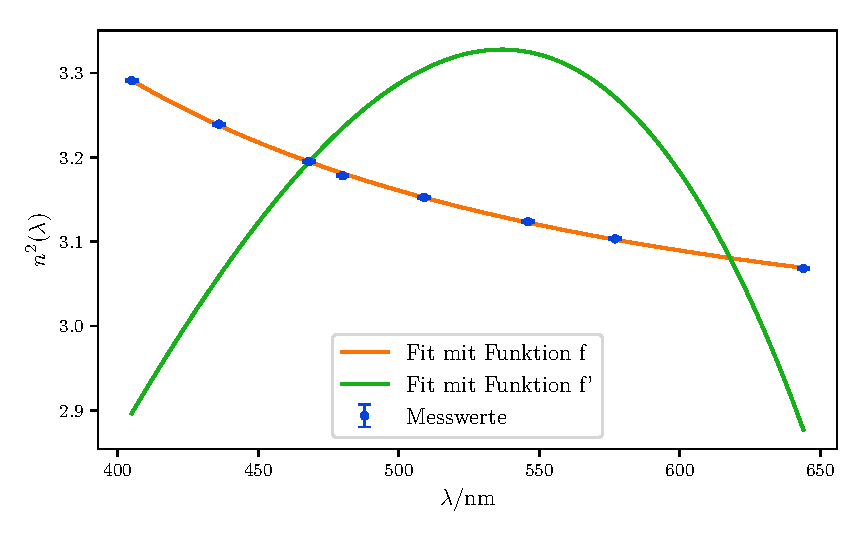
\includegraphics[width=\textwidth]{build/n.pdf}
  \caption{Dispersionskurven aus den zwei verschiedenen Ansätzen \eqref{eq:f1} und \eqref{eq:f2}.}
  \label{fig:dis}
\end{figure}
\noindent
Die Parameter ergeben sich zu:
\begin{align}
	A_0 =& \SI{2.94\pm0.01}{} \\
	A_2 =& \SI{4.97\pm0.33e4}{\per\nano\meter\squared} \\
	A_2 =& \SI{1.25\pm0.39e9}{\per\nano\meter\tothe{4}} \\
\nonumber \\
	A_2' =& \SI{-1.62\pm0.00e-5}{\per\nano\meter\squared} \\
	A_4' =& \SI{2.81\pm0.01e-11}{\per\nano\meter\tothe{4}} 
\end{align}
Die Summe der Abweichungsquadrate wird gemäß
\begin{equation}
	s^2 = \frac{1}{N-2}\sum_i^N\left(n^2(\lambda_i) - f(\lambda_i)\right)^2
\end{equation}
bestimmt.
Es ergeben sich folgende Werte:
\begin{align}
	s^2 =& \num{2.417\pm0.014e-6} \\
	{s'}^2 =& \num{5.327\pm0.011e-2} 
\end{align}
Im Folgenden wird deshalb nur die Vorschrift aus Gleichung \eqref{eq:f1} verwendet.
Aus der Herleitung von Gleichung \eqref{eq:f1} erkennt man, dass
\begin{align}
	A_0 =& \alpha + 1 \\
	A_2 =& \alpha\lambda_1^2 \\
	\lambda_1 =& \sqrt{\frac{A_2}{A_0 - 1}} 
\end{align}
gelten muss und außerdem
\begin{align}
	A_2 =& \alpha\lambda_1^2 \\
	A_4 =& \alpha\lambda_1^4 \\
	\lambda_1 =& \sqrt{\frac{A_4}{A_2}}, 
\end{align}
wobei die unphysikalischen Lösungen $\lambda_1 = 0$ und $\lambda_1 < 0$ außer Acht gelassen werden.
Aus den Ansätzen ergibt sich jeweils ein Wert von:
\begin{align}
	\lambda_1 =& \SI{160\pm5}{\nano\meter} \\
	\lambda_1 =& \SI{159\pm25}{\nano\meter} 
\end{align}
Die Abbesche Zahl, ein Maß für die Farbzersteruung, berechnet sich wie folgt:
\begin{equation}
	\nu = \frac{n(\SI{589}{\nano\meter})-1}{n(\SI{486}{\nano\meter})-n(\SI{656}{\nano\meter})}
\end{equation}
Mit der zuvor bestimmten Dispersionsfunktion ergibt sich ein Wert von:
\begin{equation}
	\nu = \num{19.0\pm1.3}
\end{equation}
Das Auflösungsvermögen gibt an, wie nah zwei Wellenlängen sich sein dürfen, damit sie immernoch unterscheidbar sind.
Es ist definiert durch
\begin{equation}
	A := \frac{\lambda}{\symup\Delta\lambda} = b\frac{\symup dn}{\symup{d\lambda}},
\end{equation}
wobei $b=\SI{3}{\centi\meter}$\cite{v402} die Basislänge des Prismas darstellt.
Es ergeben sich beispielhaft Werte für $A$ von:
\begin{align}
	A(\SI{656}{\nano\meter}) =& \num{-1.18\pm0.08e4} \\ 
	A(\SI{486}{\nano\meter}) =& \num{-3.15\pm0.24e4} 
\end{align}

\section{Diskussion}
\label{sec:Diskussion}
Wie an der Unsicherheit von $\phi$, welche unter \SI{0.04}{\percent} liegt, zu sehen ist, kann mittels eines Goniometers ein Winkel sehr genau bestimmt werden.
Somit können auch die Brechungsindices sehr genau bestimmt werden und der Unsicherheit liegt im Berech von \SI{0.01}{\percent}.
Anhand der Graphen der optimierten Näherungsfunktionen, lässt sich bereits klar sagen, dass Gleichung \eqref{eq:f2} nicht geeignet ist, um die Dispersion zu nähern.
Die Fehlerquadrate unterstützen dies deutlich, durch einen Unterschied von vier Größenordnungen.
Die Absorbtionsfrequenz lässt sich aus den Parametern der Dispersionsfunktion bestimmen. 
Da dies auf zwei Wege möglich ist und beide Ergebnisse nah beienander liegen, ist davon auszugehen, dass sich der tatsächliche Wert nah bei diesen befindet.
Jedoch ist anzumerken, dass unter Verwendung der Koeffizienten höherer Ordnung eine größere Unsicherheit auftritt.
Die Abbesche Zahl lässt sich leider nicht direkt aus den Messwerten bestimmen, da aufgrund der Art der Lichtquelle die Fraunhoferlinien nicht zu beobachten waren.
Jedoch lässt sie sich mit relativ geringer Unsicherheit aus der Dispersionsfunktion bestimmen.
Auch das Auflösungsvermögen kann mit kleiner Unsicherheit bestimmt werden.


\printbibliography{}

\end{document}
